\apendice{Especificación de Requisitos}

\section{Introducción}
En este apartado se definen los objetivos y requisitos que tiene la aplicación, analizando tanto los requisitos funcionales como no funcionales, con sus respectivos casos de uso.

\section{Objetivos generales}
Los objetivos generales establecidos para el desarrollo del proyecto son los siguientes:

\begin{itemize}
    \item Desarrollar una aplicación web que permita a los usuarios consultar, puntuar, comentar y añadir juegos docentes, según el rol que tengan en la plataforma.
    \item Conectarse a una base de datos para almacenar toda la información relacionada con los juegos y los usuarios en ella, lo que permitirá una gestión más eficiente y organizada de los datos, así como un acceso rápido y sencillo a los mismos.
    \item Implementar un sistema de búsqueda y filtros para facilitar la localización de los juegos docentes dentro de la aplicación.
    \item Asegurar que la aplicación web tenga una interfaz intuitiva, fácil de usar y atractiva para los usuarios.
    \item Realizar pruebas rigurosas para asegurarse de que la aplicación funciona correctamente y cumple con todos los requisitos del proyecto.
\end{itemize}

\section{Catalogo de requisitos}
En este apartado se definen los requisitos funcionales y no funcionales del proyecto.

\subsection{Requisitos funcionales}
Los requisitos funcionales son las tareas y funciones que debe efectuar un sistema para satisfacer las necesidades del usuario.

El proyecto tiene los siguientes requisitos funcionales:
\begin{itemize}
\tightlist
    \item \textbf{RF1-Ver acerca de:} la aplicación debe redireccionar, a través de su respectivo botón, a la página 'Acerca de', donde se mostrará información general sobre la aplicación.
    \item \textbf{RF2-Registrarse:} la aplicación debe permitir a los usuarios registrarse, creando una nueva cuenta y almacenando sus datos de registro en la base de datos del sistema.
    \item \textbf{RF3-Iniciar sesión:} la aplicación debe permitir que un usuario acceda a las funcionalidades del sistema, ingresando sus credenciales de acceso, y detectando el rol del usuario para proporcionar acceso a sus correspondientes funcionalidades.
    \item \textbf{RF4-Ver menú juegos usuario:} si el usuario identificado tiene asignado el rol de usuario, la aplicación debe proporcionar tarjetas de información de los juegos, mostrando el nombre, descripción, idioma, puntuación, enlace y valoración correspondiente de cada juego en el menú de juegos del sistema, con sus respectivas funcionalidades.
        \begin{itemize}
        \tightlist
            \item \textbf{RF4.1-Visualizar información:} los usuarios deben poder visualizar toda la información de cada juego docente.
            \item \textbf{RF4.2-Visualizar valoraciones:} los usuarios deben poder visualizar las valoraciones de cada juego docente.
            \item \textbf{RF4.3-Escribir una opinión:} los usuarios deben poder agregar una valoración a cada juego, puntuándolo y dejando una reseña.
            \item \textbf{RF4.4-Solicitar rol:} los usuarios deben poder solicitar tener el rol de profesor.
            \item \textbf{RF4.5-Buscar en barra de búsqueda:} los usuarios deben poder introducir texto en el sistema para realizar una búsqueda y ver los resultados correspondientes.
            \item \textbf{RF4.6-Filtrar por idioma del juego:} los usuarios deben poder aplicar un filtro por idioma en la búsqueda de juegos en el sistema.
            \item\textbf{RF4.7-Filtrar por puntuación del juego:} los usuarios deben poder aplicar un filtro por puntuación en la búsqueda de juegos en el sistema.
        \end{itemize}
    \item \textbf{RF5-Ver menú de juegos administrador:} si el usuario identificado tiene asignado el rol de administrador, la aplicación debe proporcionar tarjetas de información de los juegos, mostrando el nombre, descripción, idioma, puntuación, enlace y valoración correspondiente de cada juego en el menú de juegos del sistema, con sus respectivas funcionalidades.
        \begin{itemize}
        \tightlist
            \item \textbf{RF5.1-Visualizar información:} el administrador debe poder visualizar toda la información de cada juego docente.
            \item \textbf{RF5.2-Visualizar valoraciones:} el administrador debe poder visualizar las valoraciones de cada juego docente.
            \item \textbf{RF5.3-Eliminar juego:} el administrador debe poder eliminar juegos docentes marcando como borrando el juego docente en la base de datos del sistema.
            \item \textbf{RF5.4-Eliminar usuario:} el administrador debe poder eliminar usuarios marcando como borrado el usuario en la base de datos del sistema.
            \item \textbf{RF5.5-Gestionar solicitudes:} el administrador debe poder gestionar las solicitudes de rol pendientes, aceptándolas o rechazándolas.
            \item \textbf{RF5.6-Buscar en barra de búsqueda:} el administrador debe poder introducir texto en el sistema para realizar una búsqueda y ver los resultados correspondientes.
            \item \textbf{RF5.7-Filtrar por idioma del juego:} el administrador debe poder aplicar un filtro por idioma en la búsqueda de juegos en el sistema.
            \item\textbf{RF5.8-Filtrar por puntuación del juego:} el administrador debe poder aplicar un filtro por puntuación en la búsqueda de juegos en el sistema.
        \end{itemize}
    \item \textbf{RF6-Ver menú de juegos profesor:} si el usuario identificado tiene asignado el rol de profesor, la aplicación debe proporcionar tarjetas de información de los juegos, mostrando el nombre, descripción, idioma, puntuación, enlace y valoración correspondiente de cada juego en el menú de juegos del sistema, con sus respectivas funcionalidades.
        \begin{itemize}
        \tightlist
            \item \textbf{RF6.1-Visualizar información:} los profesores deben poder visualizar toda la información de cada juego docente.
            \item \textbf{RF6.2-Visualizar valoraciones:} los profesores deben poder visualizar las valoraciones de cada juego docente.
            \item \textbf{RF6.3-Añadir nuevo juego:} los profesores deben poder añadir juegos docentes almacenando los datos del nuevo juego docente en la base de datos del sistema.
            \item \textbf{RF6.4-Modificar juego :} los profesores deben poder modificar los juegos docentes ya existentes en la base de datos del sistema.
            \item \textbf{RF6.5-Añadir archivos:} los profesores deben poder añadir archivos.
            \item \textbf{RF6.6-Buscar en barra de búsqueda:} los profesores deben poder introducir texto en el sistema para realizar una búsqueda y ver los resultados correspondientes.
            \item \textbf{RF6.7-Filtrar por idioma del juego:} los profesores deben poder aplicar un filtro por idioma en la búsqueda de juegos en el sistema.
            \item\textbf{RF6.8-Filtrar por puntuación del juego:} los profesores deben poder aplicar un filtro por puntuación en la búsqueda de juegos en el sistema.
        \end{itemize}
    \item \textbf{RF7-Cambiar idioma:} el usuario debe poder modificar el idioma de la aplicación.
    \item \textbf{RF8-Ver ayuda:} el usuario debe poder ver la ayuda que proporciona el manual de usuario.
    \item \textbf{RF9-Cerrar sesión:} el usuario debe poder cerrar la sesión de su cuenta.
\end{itemize}

\subsection{Requisitos no funcionales}
Los requisitos no funcionales son las características que no están directamente asociadas con las tareas determinadas del sistema.

El proyecto tiene los siguientes requisitos no funcionales:
\begin{itemize}
\tightlist
    \item \textbf{RNF1-Usabilidad:} la aplicación debe ser fácil de usar para que los usuarios puedan utilizar todas las funcionalidades sin dificultad, proporcionando menús y opciones intuitivas y bien organizadas.
    \item \textbf{RNF2-Rendimiento:} la aplicación debe ser eficiente y garantizar tiempos de respuesta rápidos.
    \item \textbf{RNF3-Disponibilidad:} la aplicación debe estar disponible para todos los usuarios en todo momento.
    \item \textbf{RNF4-Seguridad:} la aplicación debe tener el acceso y manejo de datos confidenciales protegido y garantizar que solo los usuarios autorizados tengan acceso al sistema.
    \item \textbf{RNF5-Escalabilidad:} la aplicación debe garantizar que el sistema se adapte a futuras actualizaciones y mejoras para que pueda evolucionar considerando las necesidades de los usuarios.
    \item \textbf{RNF6-Compatibilidad:} la aplicación debe ser compatible con diferentes navegadores web y dispositivos permitiendo que los usuarios siempre tengan acceso a ella.
    \item \textbf{RNF6-Internacionalización:} la aplicación debe soportar varios idiomas, permitiendo a los usuarios seleccionar el idioma en el que desean interactuar con la aplicación. 
\end{itemize}

\section{Especificación de requisitos}
En este apartado se definen las tablas de casos de uso que especifican los requerimientos funcionales del sistema para validarlos.

\subsection{Diagrama de casos de uso}
A continuación, se muestra el diagrama de casos de uso resultante.
\begin{landscape}
\begin{figure}[h]
    \advance\leftskip-4cm \rightskip5cm
    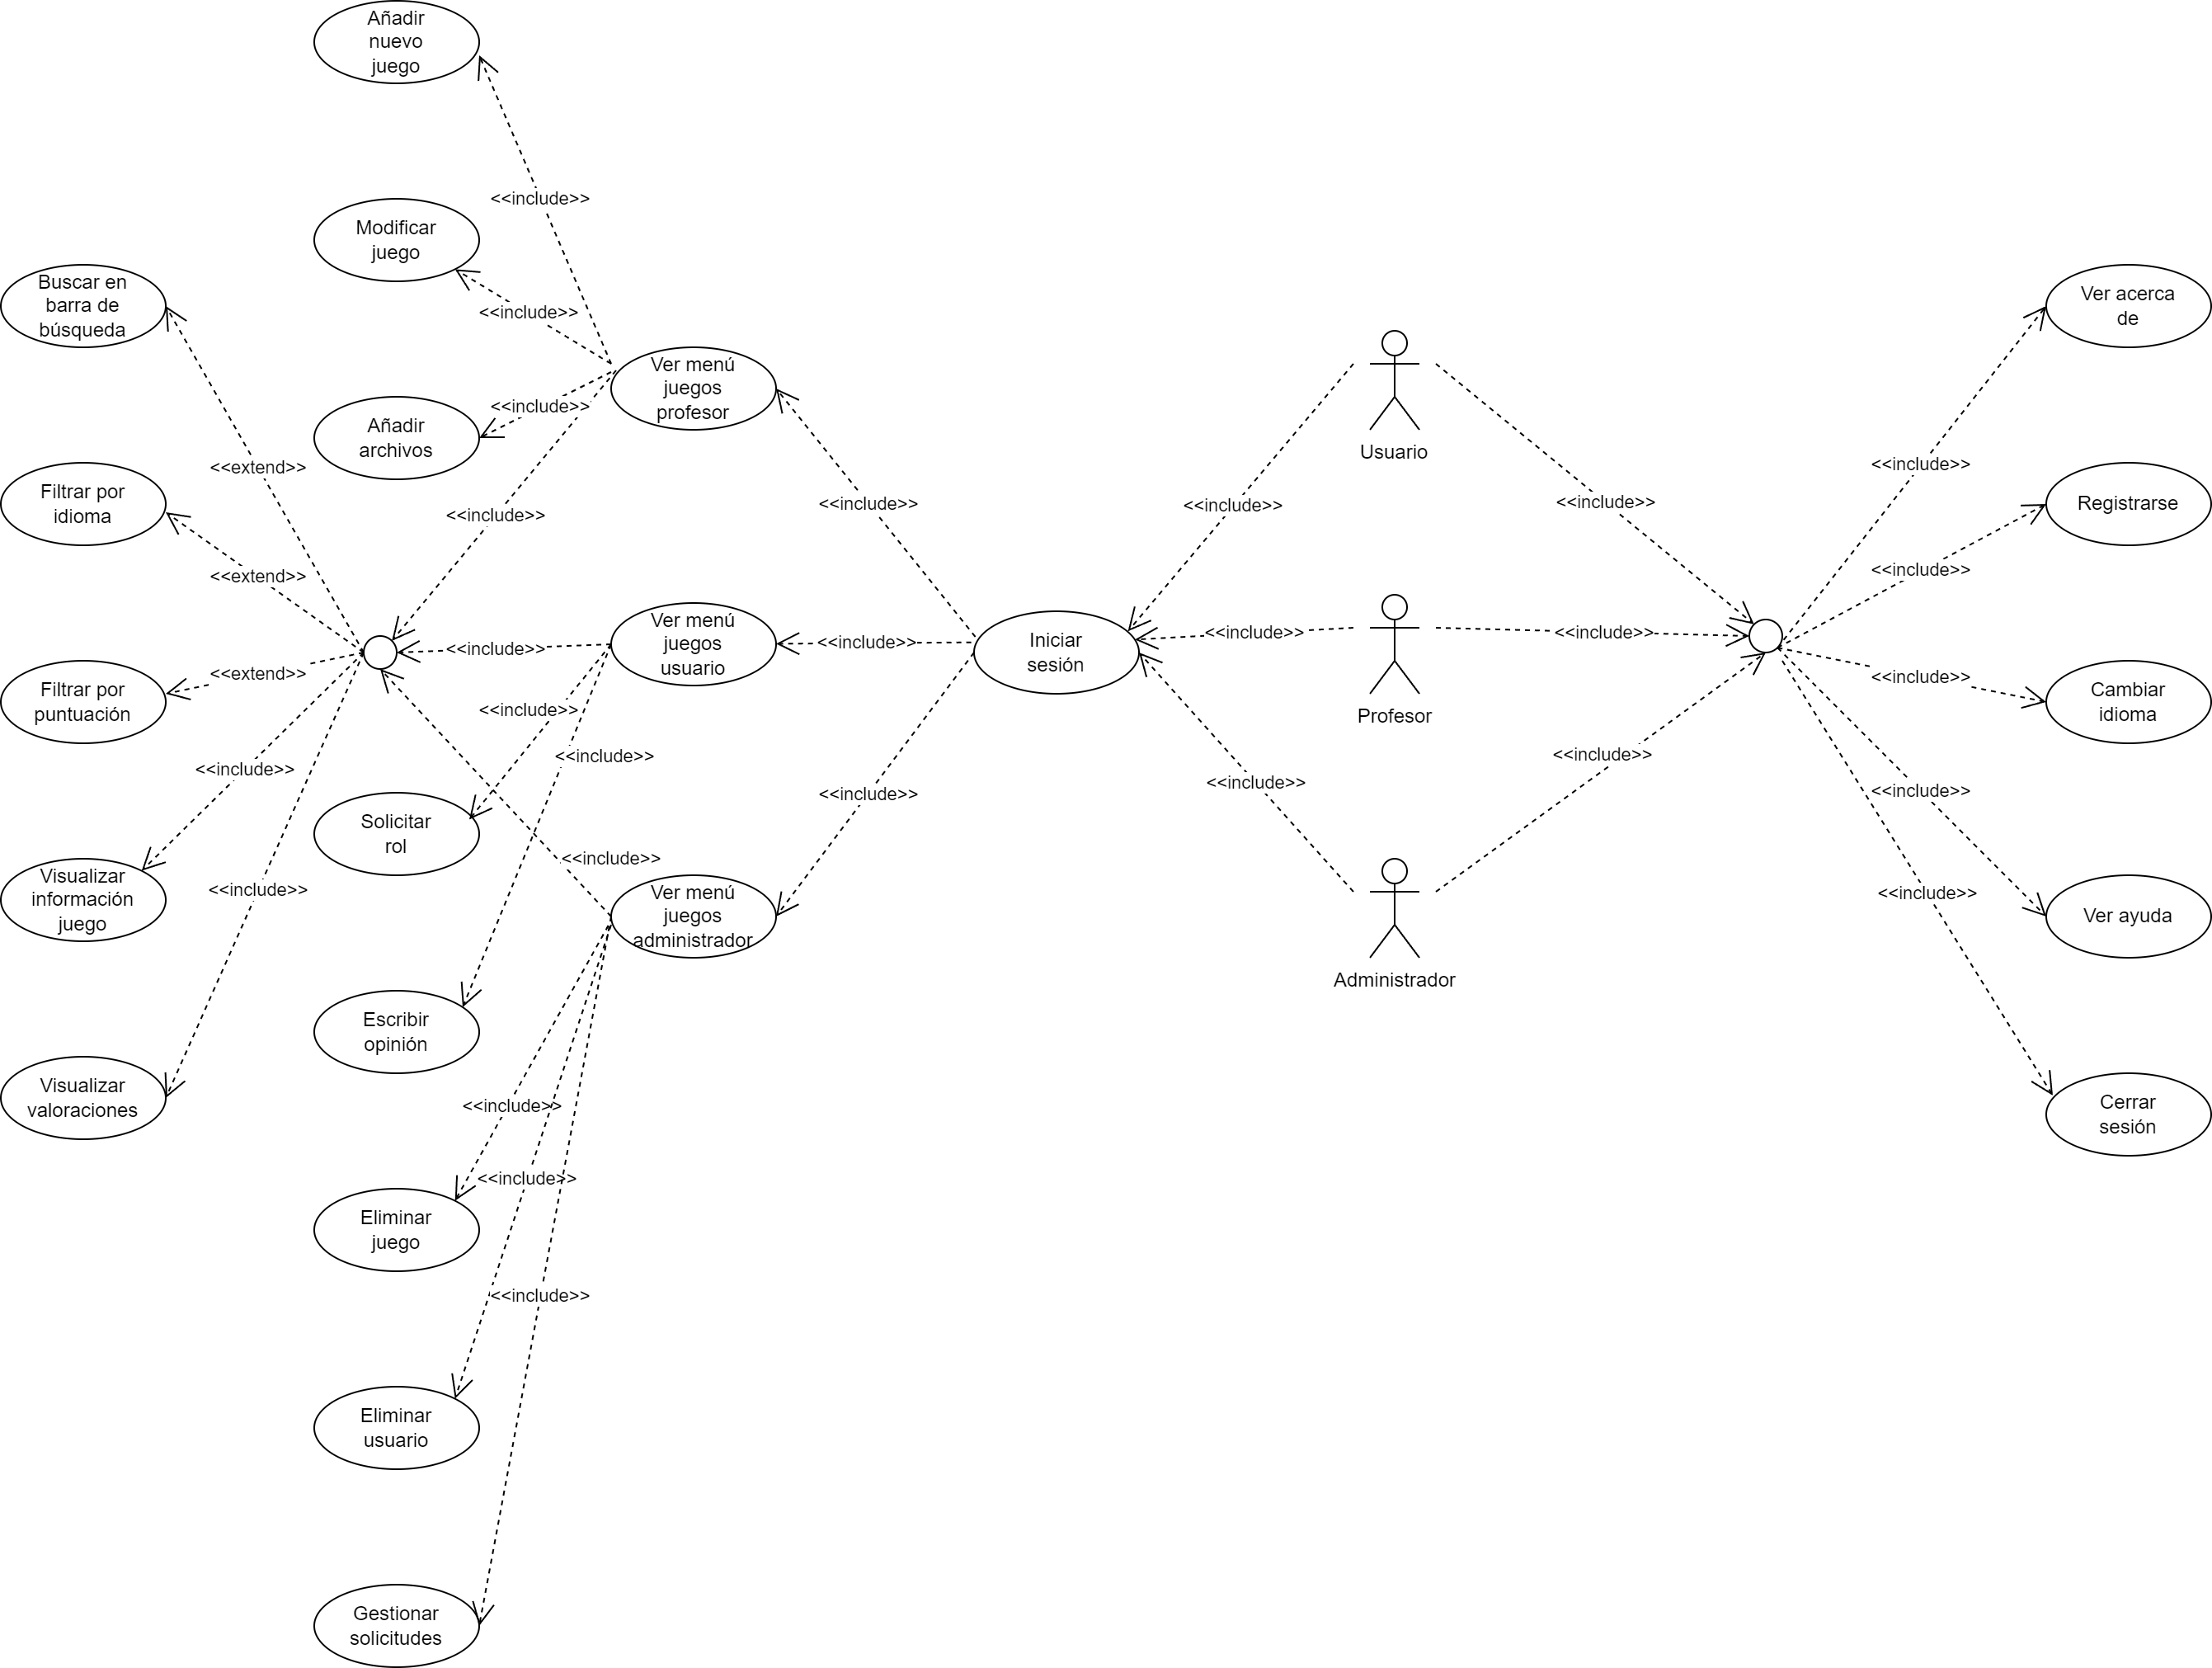
\includegraphics[scale=0.24]{img/diagrama-casos-uso.png}
    \caption{Diagrama de casos de uso}
\end{figure}
\end{landscape}

\subsection{Tablas de casos de uso}
Las tablas de casos de uso del proyecto son las siguientes:
% Caso de Uso 1 -> Ver acerca de.
\begin{table}[h!]
	\centering
	\begin{tabularx}{\linewidth}{ p{0.21\columnwidth} p{0.71\columnwidth} }
		\toprule
		\textbf{CU-01}    & \textbf{Ver acerca de}\\
		\toprule
		\textbf{Versión}              & 1.0    \\
		\textbf{Autor}                & Usuario, profesor y administrador. \\
		\textbf{Requisitos asociados} & RF-1\\
		\textbf{Descripción}          & Permite al usuario obtener información general acerca de la aplicación. \\
		\textbf{Precondiciones}         & - \\
		\textbf{Acciones}             &
		\begin{enumerate}
			\def\labelenumi{\arabic{enumi}.}
			\tightlist
			\item El usuario pulsa el botón de acerca de en la cabecera.
		\end{enumerate}\\
         \textbf{Postcondición}             & - \\
		\textbf{Excepciones}             & - \\
		\textbf{Importancia}          & Baja. \\
		\bottomrule
	\end{tabularx}
	\caption{CU-01 Ver acerca de.}
\end{table}

% Caso de Uso 2 ->Registrarse.
\begin{table}[h!]
	\centering
	\begin{tabularx}{\linewidth}{ p{0.21\columnwidth} p{0.71\columnwidth} }
		\toprule
		\textbf{CU-02}    & \textbf{Registrarse}\\
		\toprule
		\textbf{Versión}              & 1.0    \\
		\textbf{Autor}                & Usuario \\
		\textbf{Requisitos asociados} & RF-2\\
		\textbf{Descripción}          & Permite al usuario registrar su nueva cuenta. \\
		\textbf{Precondiciones}         & La base de datos debe estar disponible. \\
		\textbf{Acciones}             &
		\begin{enumerate}
			\def\labelenumi{\arabic{enumi}.}
			\tightlist
			\item El usuario accede a la opción de registrarse.
			\item El usuario introduce su nombre de usuario, nombre, apellido, institución y contraseña.
            \item El usuario pulsa el botón de crear cuenta.
		\end{enumerate}\\
         \textbf{Postcondiciones}             &
		\begin{enumerate}
			\def\labelenumi{\arabic{enumi}.}
			\tightlist
			\item El nombre del usuario no debe existir en la base de datos.
			\item La contraseña debe contener al menos 8 caracteres, una mayúscula, una minúscula y un símbolo.
            \item Todos los campos deben ser rellenados excepto el de la institución que es opcional.
		\end{enumerate}\\
		\textbf{Excepciones}             &
		\begin{enumerate}
			\def\labelenumi{\arabic{enumi}.}
			\tightlist
			\item El nombre de usuario ya existe (mensaje).
			\item El campo es requerido (mensaje).
            \item La contraseña debe contener al menos 8 caracteres, una mayúscula, una minúscula y un símbolo (mensaje).
            \item Las contraseñas ingresadas no coinciden (mensaje).
		\end{enumerate}\\
		\textbf{Importancia}          & Alta. \\
		\bottomrule
	\end{tabularx}
	\caption{CU-02 Registrarse.}
\end{table}


% Caso de Uso 3 -> Iniciar sesión.
\begin{table}[h!]
	\centering
	\begin{tabularx}{\linewidth}{ p{0.21\columnwidth} p{0.71\columnwidth} }
		\toprule
		\textbf{CU-03}    & \textbf{Iniciar sesión}\\
		\toprule
		\textbf{Versión}              & 1.0    \\
		\textbf{Autor}                & Usuario, profesor y administrador. \\
		\textbf{Requisitos asociados} & RF-3\\
		\textbf{Descripción}          & Permite al usuario iniciar sesión de su cuenta. \\
		\textbf{Precondiciones}         & El usuario debe estar registrado. \\
		\textbf{Acciones}             &
		\begin{enumerate}
			\def\labelenumi{\arabic{enumi}.}
			\tightlist
			\item El usuario accede a la opción de iniciar sesión o comenzar.
			\item El usuario introduce su nombre de usuario y contraseña.
            \item El usuario pulsa el botón de Iniciar sesión.
            \item El sistema verifica y autentica las credenciales del usuario.
		\end{enumerate}\\
         \textbf{Postcondiciones}             &
		\begin{enumerate}
			\def\labelenumi{\arabic{enumi}.}
			\tightlist
			\item El nombre del usuario y la contraseña deben existir en la base de datos.
		\end{enumerate}\\
		\textbf{Excepciones}             &
		\begin{enumerate}
			\def\labelenumi{\arabic{enumi}.}
			\tightlist
			\item El nombre de usuario o contraseña no son correctos (mensaje).
			\item Ha introducido la contraseña incorrecta más de tres veces. Cuenta bloqueada. (mensaje).
		\end{enumerate}\\
		\textbf{Importancia}          & Alta. \\
		\bottomrule
	\end{tabularx}
	\caption{CU-03 Iniciar sesión.}
\end{table}

% Caso de Uso 4 -> Ver menú juegos usuario.
\begin{table}[h!]
	\centering
	\begin{tabularx}{\linewidth}{ p{0.21\columnwidth} p{0.71\columnwidth} }
		\toprule
		\textbf{CU-04}    & \textbf{Ver menú juegos usuario}\\
		\toprule
		\textbf{Versión}              & 1.0    \\
		\textbf{Autor}                & Usuario. \\
		\textbf{Requisitos asociados} & RF-4, RF-4.1, RF.4.2, RF.4.3, RF.4.4, RF.4.5, RF.4.6, RF.4.7 \\
		\textbf{Descripción}          & Permite al usuario navegar por el menú de juegos, permitiéndole hacer búsquedas, aplicar filtros y ver más información y las valoraciones de los juegos, añadir una opinión y solicitar el rol de profesor.\\
		\textbf{Precondiciones}         & El usuario debe haber iniciado sesión como usuario. \\
		\textbf{Acciones}             &
		\begin{enumerate}
			\def\labelenumi{\arabic{enumi}.}
			\tightlist
			\item El usuario inicia sesión.
            \item El sistema verifica y autentica las credenciales del usuario.
            \item El usuario es redireccionado al menú de juegos.
            \item El sistema muestra las tarjetas de información de los juegos disponibles.
            \item El usuario puede realizar una búsqueda mediante barra de búsqueda o por filtros.
            \item El sistema puede mostrar los resultados de acuerdo con la búsqueda.
            \item El profesor puede pulsar el botón de ver más información del juego.
            \item El profesor puede pulsar el botón de ver las valoraciones del juego.
            \item El usuario puede añadir una opinión a cada juego.
            \item El usuario puede pulsar el botón de contacto para solicitar el rol de profesor.
		\end{enumerate}\\
         \textbf{Postcondición}             & El resultado de la búsqueda debe existir en la base de datos. \\
		\textbf{Excepciones}             &
		\begin{enumerate}
			\def\labelenumi{\arabic{enumi}.}
			\tightlist
			\item No se han encontrado resultados de búsqueda. (mensaje).
		\end{enumerate}\\
		\textbf{Importancia}          & Alta. \\
		\bottomrule
	\end{tabularx}
	\caption{CU-04 Ver menú juegos usuario.}
\end{table}

% Caso de Uso 5 -> Escribir opinión.
\begin{table}[h!]
	\centering
	\begin{tabularx}{\linewidth}{ p{0.21\columnwidth} p{0.71\columnwidth} }
		\toprule
		\textbf{CU-05}    & \textbf{Escribir opinión}\\
		\toprule
		\textbf{Versión}              & 1.0    \\
		\textbf{Autor}                & Usuario. \\
		\textbf{Requisitos asociados} & RF-4, RF.4.3 \\
		\textbf{Descripción}          & Permite al usuario escribir una opinión sobre cada juegos, puntuándolo y dejando una reseña.\\
		\textbf{Precondiciones}         & El usuario debe haber iniciado sesión como usuario. \\
		\textbf{Acciones}             &
		\begin{enumerate}
			\def\labelenumi{\arabic{enumi}.}
			\tightlist
		\item El usuario inicia sesión.
            \item El sistema verifica y autentica las credenciales del usuario.
            \item El usuario es redireccionado al menú de juegos.
            \item El usuario pulsa al botón de escribir opinión.
            \item El usuario selecciona la puntuación.
            \item El usuario escribe una reseña.
            \item El usuario pulsa el botón de enviar opinión.
            \item El usuario es redireccionado al menú de juegos.
		\end{enumerate}\\
         \textbf{Postcondición}             & - \\
		\textbf{Excepciones}             & - \\
		\textbf{Importancia}          & Media. \\
		\bottomrule
	\end{tabularx}
	\caption{CU-05 Escribir opinión.}
\end{table}

% Caso de Uso 6 -> Solicitar rol.
\begin{table}[h!]
	\centering
	\begin{tabularx}{\linewidth}{ p{0.21\columnwidth} p{0.71\columnwidth} }
		\toprule
		\textbf{CU-06}    & \textbf{Solicitar rol}\\
		\toprule
		\textbf{Versión}              & 1.0    \\
		\textbf{Autor}                & Usuario. \\
		\textbf{Requisitos asociados} & RF-4, RF.4.4 \\
		\textbf{Descripción}          & Permite al usuario solicitar el rol de profesor.\\
		\textbf{Precondiciones}         & El usuario debe haber iniciado sesión como usuario. \\
		\textbf{Acciones}             &
		\begin{enumerate}
			\def\labelenumi{\arabic{enumi}.}
			\tightlist
			\item El usuario inicia sesión.
            \item El sistema verifica y autentica las credenciales del usuario.
            \item El usuario es redireccionado al menú de juegos.
            \item El usuario pulsa al botón de contacto.
            \item El sistema muestra un mensaje con la explicación de cómo solicitar el rol.
            \item El usuario pulsa el botón de solicitar rol.
            \item El sistema muestra un mensaje de éxito
		\end{enumerate}\\
         \textbf{Postcondición}             & - \\
		\textbf{Excepciones}             & - \\
		\textbf{Importancia}          & Media. \\
		\bottomrule
	\end{tabularx}
	\caption{CU-06 Solicitar rol.}
\end{table}

% Caso de Uso 7 -> Ver menú juegos administrador.
\begin{table}[h!]
	\centering
	\begin{tabularx}{\linewidth}{ p{0.21\columnwidth} p{0.71\columnwidth} }
		\toprule
		\textbf{CU-07}    & \textbf{Ver menú juegos administrador}\\
		\toprule
		\textbf{Versión}              & 1.0    \\
		\textbf{Autor}                & Administrador. \\
		\textbf{Requisitos asociados} & RF-5, RF-5.1, RF.5.2, RF.5.3, RF.5.4, RF.5.5, RF.5.6, RF.5.7, RF.5.8 \\
		\textbf{Descripción}          & Permite al administrador navegar por el menú de juegos, permitiéndole hacer búsquedas, aplicar filtros y ver más información y las valoraciones de los juegos, eliminar un usuario, eliminar un juego y gestionar las solicitudes.\\
		\textbf{Precondiciones}         & El usuario debe haber iniciado sesión como administrador. \\
		\textbf{Acciones}             &
		\begin{enumerate}
			\def\labelenumi{\arabic{enumi}.}
			\tightlist
			\item El administrador inicia sesión.
            \item El sistema verifica y autentica las credenciales del administrador.
            \item El administrador es redireccionado al menú de juegos.
            \item El sistema muestra las tarjetas de información de los juegos disponibles.
            \item El administrador puede realizar una búsqueda mediante barra de búsqueda o por filtros.
            \item El sistema puede mostrar los resultados de acuerdo con la búsqueda.
            \item El profesor puede pulsar el botón de ver más información del juego.
            \item El profesor puede pulsar el botón de ver las valoraciones del juego.
            \item El administrador puede eliminar un juego.
            \item El administrador puede eliminar un usuario.
            \item El administrador puede gestionar las solicitudes.
		\end{enumerate}\\
         \textbf{Postcondición}             & El resultado de la búsqueda debe existir en la base de datos. \\
		\textbf{Excepciones}             &
		\begin{enumerate}
			\def\labelenumi{\arabic{enumi}.}
			\tightlist
			\item No se han encontrado resultados de búsqueda. (mensaje).
		\end{enumerate}\\
		\textbf{Importancia}          & Alta. \\
		\bottomrule
	\end{tabularx}
	\caption{CU-07 Ver menú juegos administrador.}
\end{table}

% Caso de Uso 8 -> Eliminar juego.
\begin{table}[h!]
	\centering
	\begin{tabularx}{\linewidth}{ p{0.21\columnwidth} p{0.71\columnwidth} }
		\toprule
		\textbf{CU-08}    & \textbf{Eliminar juego}\\
		\toprule
		\textbf{Versión}              & 1.0    \\
		\textbf{Autor}                & Administrador. \\
		\textbf{Requisitos asociados} & RF-5, RF.5.3 \\
		\textbf{Descripción}          & Permite al usuario eliminar un juego docente del sistema.\\
		\textbf{Precondiciones}         & El usuario debe haber iniciado sesión como administrador. \\
		\textbf{Acciones}             &
		\begin{enumerate}
			\def\labelenumi{\arabic{enumi}.}
			\tightlist
			\item El administrador inicia sesión.
            \item El sistema verifica y autentica las credenciales del administrador.
            \item El administrador es redireccionado al menú de juegos.
            \item El administrador pulsa al botón de administración.
            \item El administrador pulsa al botón de gestión de juegos.
            \item El sistema muestra una lista de juegos docentes existentes.
    	\item El administrador selecciona un juego docente para eliminar.
    	\item El sistema marca el juego docente como borrado en la base de datos.
		\end{enumerate}\\
         \textbf{Postcondición}             & - \\
		\textbf{Excepciones}             & - \\
		\textbf{Importancia}          & Media. \\
		\bottomrule
	\end{tabularx}
	\caption{CU-08 Eliminar juego.}
\end{table}

% Caso de Uso 9 -> Eliminar usuario.
\begin{table}[h!]
	\centering
	\begin{tabularx}{\linewidth}{ p{0.21\columnwidth} p{0.71\columnwidth} }
		\toprule
		\textbf{CU-09}    & \textbf{Eliminar usuario}\\
		\toprule
		\textbf{Versión}              & 1.0    \\
		\textbf{Autor}                & Administrador. \\
		\textbf{Requisitos asociados} & RF-5, RF.5.4 \\
		\textbf{Descripción}          & Permite al usuario eliminar un usuario del sistema.\\
		\textbf{Precondiciones}         & El usuario debe haber iniciado sesión como administrador. \\
		\textbf{Acciones}             &
		\begin{enumerate}
			\def\labelenumi{\arabic{enumi}.}
			\tightlist
			\item El administrador inicia sesión.
            \item El sistema verifica y autentica las credenciales del administrador.
            \item El administrador es redireccionado al menú de juegos.
            \item El administrador pulsa al botón de administración.
            \item El administrador pulsa al botón de gestión de usuarios.
            \item El sistema muestra una lista de los usuarios existentes.
    	\item El administrador selecciona un usuario para eliminar.
    	\item El sistema marca el usuario como borrado en la base de datos.
		\end{enumerate}\\
         \textbf{Postcondición}             & - \\
		\textbf{Excepciones}             & - \\
		\textbf{Importancia}          & Media. \\
		\bottomrule
	\end{tabularx}
	\caption{CU-09 Eliminar usuario.}
\end{table}

% Caso de Uso 10 -> Gestionar solicitudes.
\begin{table}[h!]
	\centering
	\begin{tabularx}{\linewidth}{ p{0.21\columnwidth} p{0.71\columnwidth} }
		\toprule
		\textbf{CU-10}    & \textbf{Gestionar solicitudes}\\
		\toprule
		\textbf{Versión}              & 1.0    \\
		\textbf{Autor}                & Administrador. \\
		\textbf{Requisitos asociados} & RF-5, RF.5.5 \\
		\textbf{Descripción}          & Permite al usuario gestionar las solicitudes pendientes del sismtea.\\
		\textbf{Precondiciones}         & El usuario debe haber iniciado sesión como administrador. \\
		\textbf{Acciones}             &
		\begin{enumerate}
			\def\labelenumi{\arabic{enumi}.}
			\tightlist
			\item El administrador inicia sesión.
            \item El sistema verifica y autentica las credenciales del administrador.
            \item El administrador es redireccionado al menú de juegos.
            \item El administrador pulsa al botón de administración.
            \item El administrador pulsa al botón de gestión de solicitudes.
            \item El sistema muestra una lista de las solicitudes pendientes.
    	\item El administrador acepta o rechaza una solicitud.
    	\item El sistema marca la solicitud como aceptada o rechazada en la base de datos.
		\end{enumerate}\\
         \textbf{Postcondición}             & - \\
		\textbf{Excepciones}             & - \\
		\textbf{Importancia}          & Media. \\
		\bottomrule
	\end{tabularx}
	\caption{CU-10 Gestionar solicitudes.}
\end{table}

% Caso de Uso 11 -> Ver menú juegos profesor.
\begin{table}[h!]
	\centering
	\begin{tabularx}{\linewidth}{ p{0.21\columnwidth} p{0.71\columnwidth} }
		\toprule
		\textbf{CU-11}    & \textbf{Ver menú juegos profesor}\\
		\toprule
		\textbf{Versión}              & 1.0    \\
		\textbf{Autor}                & Profesor. \\
		\textbf{Requisitos asociados} & RF-6, RF-6.1, RF.6.2, RF.6.3, RF.6.4, RF.6.5, RF.6.6, RF.6.7, RF.6.8 \\
		\textbf{Descripción}          & Permite al profesor navegar por el menú de juegos, permitiéndole hacer búsquedas, aplicar filtros y ver más información y las valoraciones de los juegos, añadir un nuevo juego, modificar un juego existente y añadir archivos a los juegos.\\
		\textbf{Precondiciones}         & El usuario debe haber iniciado sesión como profesor. \\
		\textbf{Acciones}             &
		\begin{enumerate}
			\def\labelenumi{\arabic{enumi}.}
			\tightlist
			\item El profesor inicia sesión.
            \item El sistema verifica y autentica las credenciales del profesor.
            \item El profesor es redireccionado al menú de juegos.
            \item El sistema muestra las tarjetas de información de los juegos disponibles.
            \item El profesor puede realizar una búsqueda mediante barra de búsqueda o por filtros.
            \item El sistema puede mostrar los resultados de acuerdo con la búsqueda.
            \item El profesor puede pulsar el botón de ver más información del juego.
            \item El profesor puede pulsar el botón de ver las valoraciones del juego.
            \item El profesor puede añadir un nuevo juego.
            \item El profesor puede modificar un juego.
            \item El profesor puede añadir archivos a los juegos.
		\end{enumerate}\\
         \textbf{Postcondición}             & El resultado de la búsqueda debe existir en la base de datos. \\
		\textbf{Excepciones}             &
		\begin{enumerate}
			\def\labelenumi{\arabic{enumi}.}
			\tightlist
			\item No se han encontrado resultados de búsqueda. (mensaje).
		\end{enumerate}\\
		\textbf{Importancia}          & Alta. \\
		\bottomrule
	\end{tabularx}
	\caption{CU-11 Ver menú juegos profesor.}
\end{table}

% Caso de Uso 12 -> Añadir nuevo juego.
\begin{table}[h!]
	\centering
	\begin{tabularx}{\linewidth}{ p{0.21\columnwidth} p{0.71\columnwidth} }
		\toprule
		\textbf{CU-12}    & \textbf{Añadir nuevo juego}\\
		\toprule
		\textbf{Versión}              & 1.0    \\
		\textbf{Autor}                & Profesor. \\
		\textbf{Requisitos asociados} & RF-6, RF.6.3 \\
		\textbf{Descripción}          & Permite al profesor añadir un nuevo juego.\\
		\textbf{Precondiciones}         & El usuario debe haber iniciado sesión como profesor. \\
		\textbf{Acciones}             &
		\begin{enumerate}
			\def\labelenumi{\arabic{enumi}.}
			\tightlist
			\item El profesor inicia sesión.
            \item El sistema verifica y autentica las credenciales del profesor.
            \item El profesor es redireccionado al menú de juegos.
            \item El profesor pulsa el botón de añadir juego.
            \item El sistema muestra un formulario para ingresar los datos del nuevo juego.
    	\item El profesor completa los campos del formulario.
    	\item El sistema almacena los datos del nuevo juego en la base de datos.
		\end{enumerate}\\
         \textbf{Postcondición}             & Todos los campos requeridos deben ser rellenados. \\
		\textbf{Excepciones}             & - \\
		\textbf{Importancia}          & Alta. \\
		\bottomrule
	\end{tabularx}
	\caption{CU-12 Añadir nuevo juego.}
\end{table}

% Caso de Uso 13 -> Modificar juego.
\begin{table}[h!]
	\centering
	\begin{tabularx}{\linewidth}{ p{0.21\columnwidth} p{0.71\columnwidth} }
		\toprule
		\textbf{CU-13}    & \textbf{Modificar juego}\\
		\toprule
		\textbf{Versión}              & 1.0    \\
		\textbf{Autor}                & Profesor. \\
		\textbf{Requisitos asociados} & RF-6, RF.6.4 \\
		\textbf{Descripción}          & Permite al profesor modificar un juego ya existente.\\
		\textbf{Precondiciones}         & El usuario debe haber iniciado sesión como profesor. \\
		\textbf{Acciones}             &
		\begin{enumerate}
			\def\labelenumi{\arabic{enumi}.}
			\tightlist
			\item El profesor inicia sesión.
            \item El sistema verifica y autentica las credenciales del profesor.
            \item El profesor es redireccionado al menú de juegos.
    	\item El profesor selecciona un juego docente para modificar.
            \item El profesor pulsa el botón de modificar juego.
    	\item El sistema muestra el formulario con los datos actuales del juego.
    	\item El profesor realiza las modificaciones necesarias en el formulario.
            \item El sistema actualiza los datos del juego docente en la base de datos.
		\end{enumerate}\\
         \textbf{Postcondición}             & Todos los campos requeridos deben ser rellenados. \\
		\textbf{Excepciones}             & - \\
		\textbf{Importancia}          & Alta. \\
		\bottomrule
	\end{tabularx}
	\caption{CU-13 Modificar juego.}
\end{table}

% Caso de Uso 14 -> Añadir archivos.
\begin{table}[h!]
	\centering
	\begin{tabularx}{\linewidth}{ p{0.21\columnwidth} p{0.71\columnwidth} }
		\toprule
		\textbf{CU-14}    & \textbf{Añadir archivos}\\
		\toprule
		\textbf{Versión}              & 1.0    \\
		\textbf{Autor}                & Profesor. \\
		\textbf{Requisitos asociados} & RF-6, RF.6.5 \\
		\textbf{Descripción}          & Permite al profesor añadir archivos a los juegos.\\
		\textbf{Precondiciones}         & El usuario debe haber iniciado sesión como profesor. \\
		\textbf{Acciones}             &
		\begin{enumerate}
			\def\labelenumi{\arabic{enumi}.}
			\tightlist
			\item El profesor inicia sesión.
            \item El sistema verifica y autentica las credenciales del profesor.
            \item El profesor es redireccionado al menú de juegos.
    	\item El profesor selecciona un juego docente al que añadir archivos.
            \item El sistema muestra una interfaz de carga de archivos.
    	\item El profesor selecciona uno o varios archivos y los sube al sistema.
    	\item El sistema almacena los archivos en el sistema.
		\end{enumerate}\\
         \textbf{Postcondición}             & - \\
		\textbf{Excepciones}             & - \\
		\textbf{Importancia}          & Media. \\
		\bottomrule
	\end{tabularx}
	\caption{CU-14 Añadir archivos.}
\end{table}

% Caso de Uso 15 -> Buscar en barra de búsqueda.
\begin{table}[h!]
	\centering
	\begin{tabularx}{\linewidth}{ p{0.21\columnwidth} p{0.71\columnwidth} }
		\toprule
		\textbf{CU-15}    & \textbf{Buscar en barra de búsqueda}\\
		\toprule
		\textbf{Versión}              & 1.0    \\
		\textbf{Autor}                & Usuario, profesor y administrador. \\
		\textbf{Requisitos asociados} & RF-4, RF-4.5, RF-5, RF-5.6, RF-6, RF-6.6 \\
		\textbf{Descripción}          & Permite al usuario, profesor o administrado buscar juegos mediante la barra de búsqueda.\\
		\textbf{Precondiciones}         & El usuario debe haber iniciado sesión. \\
		\textbf{Acciones}             &
		\begin{enumerate}
			\def\labelenumi{\arabic{enumi}.}
			\tightlist
			\item El usuario inicia sesión.
            \item El sistema verifica y autentica las credenciales del usuario.
            \item El usuario es redireccionado al menú de juegos.
            \item El sistema muestra una barra de búsqueda y opciones de filtro por idioma y puntuación.
            \item El usuario puede introducir texto en la barra de búsqueda para realizar una búsqueda personalizada.
            \item El sistema muestra los resultados correspondientes a la búsqueda realizada.
		\end{enumerate}\\
         \textbf{Postcondición}             & El resultado de la búsqueda debe existir en la base de datos. \\
		\textbf{Excepciones}             &
		\begin{enumerate}
			\def\labelenumi{\arabic{enumi}.}
			\tightlist
			\item No se han encontrado resultados de búsqueda. (mensaje).
		\end{enumerate}\\
		\textbf{Importancia}          & Media. \\
		\bottomrule
	\end{tabularx}
	\caption{CU-15 Buscar en barra de búsqueda.}
\end{table}

% Caso de Uso 16 -> Filtrar por idioma.
\begin{table}[h!]
	\centering
	\begin{tabularx}{\linewidth}{ p{0.21\columnwidth} p{0.71\columnwidth} }
		\toprule
		\textbf{CU-16}    & \textbf{Filtrar por idioma}\\
		\toprule
		\textbf{Versión}              & 1.0    \\
		\textbf{Autor}                & Usuario, profesor y administrador. \\
		\textbf{Requisitos asociados} & RF-4, RF-4.6, RF-5, RF-5.7, RF-6, RF-6.7 \\
		\textbf{Descripción}          & Permite al usuario, profesor o administrado buscar juegos mediante la aplicación de filtros por idioma.\\
		\textbf{Precondiciones}         & El usuario debe haber iniciado sesión. \\
		\textbf{Acciones}             &
		\begin{enumerate}
			\def\labelenumi{\arabic{enumi}.}
			\tightlist
			\item El usuario inicia sesión.
            \item El sistema verifica y autentica las credenciales del usuario.
            \item El usuario es redireccionado al menú de juegos.
            \item El sistema muestra una barra de búsqueda y opciones de filtro por idioma y puntuación.
            \item El usuario de aplicar filtros por idioma para refinar la búsqueda.
            \item El sistema filtra los juegos según los criterios seleccionados y muestra los resultados actualizados.
		\end{enumerate}\\
         \textbf{Postcondición}             & El resultado de la búsqueda debe existir en la base de datos. \\
		\textbf{Excepciones}             &
		\begin{enumerate}
			\def\labelenumi{\arabic{enumi}.}
			\tightlist
			\item No se han encontrado resultados de búsqueda. (mensaje).
		\end{enumerate}\\
		\textbf{Importancia}          & Media. \\
		\bottomrule
	\end{tabularx}
	\caption{CU-16 Filtrar por idioma.}
\end{table}

% Caso de Uso 17 -> Filtrar por puntuación.
\begin{table}[h!]
	\centering
	\begin{tabularx}{\linewidth}{ p{0.21\columnwidth} p{0.71\columnwidth} }
		\toprule
		\textbf{CU-17}    & \textbf{Filtrar por puntuación}\\
		\toprule
		\textbf{Versión}              & 1.0    \\
		\textbf{Autor}                & Usuario, profesor y administrador. \\
		\textbf{Requisitos asociados} & RF-4, RF-4.7, RF-5, RF-5.8, RF-6, RF-6.8 \\
		\textbf{Descripción}          & Permite al usuario, profesor o administrado buscar juegos mediante la aplicación de filtros por puntuación.\\
		\textbf{Precondiciones}         & El usuario debe haber iniciado sesión. \\
		\textbf{Acciones}             &
		\begin{enumerate}
			\def\labelenumi{\arabic{enumi}.}
			\tightlist
			\item El usuario inicia sesión.
            \item El sistema verifica y autentica las credenciales del usuario.
            \item El usuario es redireccionado al menú de juegos.
            \item El sistema muestra una barra de búsqueda y opciones de filtro por idioma y puntuación.
            \item El usuario de aplicar filtros por puntuación para refinar la búsqueda.
            \item El sistema filtra los juegos según los criterios seleccionados y muestra los resultados actualizados.
		\end{enumerate}\\
         \textbf{Postcondición}             & El resultado de la búsqueda debe existir en la base de datos. \\
		\textbf{Excepciones}             &
		\begin{enumerate}
			\def\labelenumi{\arabic{enumi}.}
			\tightlist
			\item No se han encontrado resultados de búsqueda. (mensaje).
		\end{enumerate}\\
		\textbf{Importancia}          & Media. \\
		\bottomrule
	\end{tabularx}
	\caption{CU-17 Filtrar por puntuación.}
\end{table}

% Caso de Uso 18 -> Visualizar información juego.
\begin{table}[h!]
	\centering
	\begin{tabularx}{\linewidth}{ p{0.21\columnwidth} p{0.71\columnwidth} }
		\toprule
		\textbf{CU-18}    & \textbf{Visualizar información juego}\\
		\toprule
		\textbf{Versión}              & 1.0    \\
		\textbf{Autor}                & Usuario, profesor y administrador. \\
		\textbf{Requisitos asociados} & RF-4, RF-4.1, RF-5, RF-5.1, RF-6, RF-6.1 \\
		\textbf{Descripción}          & Permite al usuario, profesor o administrado visualizar la información más detallada de los juegos.\\
		\textbf{Precondiciones}         & El usuario debe haber iniciado sesión. \\
		\textbf{Acciones}             &
		\begin{enumerate}
			\def\labelenumi{\arabic{enumi}.}
			\tightlist
			\item El usuario inicia sesión.
            \item El sistema verifica y autentica las credenciales del usuario.
            \item El usuario es redireccionado al menú de juegos.
            \item El usuario pulsa el botón de ver más información del juego deseado.
            \item El sistema muestra la información detallada del juego.
		\end{enumerate}\\
         \textbf{Postcondición}             & - \\
		\textbf{Excepciones}             & - \\
		\textbf{Importancia}          & Alta. \\
		\bottomrule
	\end{tabularx}
	\caption{CU-18 Visualizar información juego.}
\end{table}

% Caso de Uso 19 -> Visualizar valoraciones.
\begin{table}[h!]
	\centering
	\begin{tabularx}{\linewidth}{ p{0.21\columnwidth} p{0.71\columnwidth} }
		\toprule
		\textbf{CU-19}    & \textbf{Visualizar valoraciones}\\
		\toprule
		\textbf{Versión}              & 1.0    \\
		\textbf{Autor}                & Usuario, profesor y administrador. \\
		\textbf{Requisitos asociados} & RF-4, RF-4.2, RF-5, RF-5.2, RF-6, RF-6.2 \\
		\textbf{Descripción}          & Permite al usuario, profesor o administrado visualizar las valoraciones de los juegos.\\
		\textbf{Precondiciones}         & El usuario debe haber iniciado sesión. \\
		\textbf{Acciones}             &
		\begin{enumerate}
			\def\labelenumi{\arabic{enumi}.}
			\tightlist
			\item El usuario inicia sesión.
            \item El sistema verifica y autentica las credenciales del usuario.
            \item El usuario es redireccionado al menú de juegos.
            \item El usuario pulsa el botón de ver las valoraciones del juego deseado.
            \item El sistema muestra las valoraciones del juego.
		\end{enumerate}\\
         \textbf{Postcondición}             & - \\
		\textbf{Excepciones}             & - \\
		\textbf{Importancia}          & Media. \\
		\bottomrule
	\end{tabularx}
	\caption{CU-19 Visualizar valoraciones.}
\end{table}

% Caso de Uso 20 ->  Cambiar idioma.
\begin{table}[h!]
	\centering
	\begin{tabularx}{\linewidth}{ p{0.21\columnwidth} p{0.71\columnwidth} }
		\toprule
		\textbf{CU-20}    & \textbf{Cambiar idioma}\\
		\toprule
		\textbf{Versión}              & 1.0    \\
		\textbf{Autor}                & Usuario, profesor y administrador. \\
		\textbf{Requisitos asociados} & RF-7\\
		\textbf{Descripción}          & Permite al usuario cambiar el idioma de la aplicación. \\
		\textbf{Precondiciones}         & - \\
		\textbf{Acciones}             &
		\begin{enumerate}
			\def\labelenumi{\arabic{enumi}.}
			\tightlist
			\item El sistema muestra las opciones de idioma.
			\item El usuario selecciona el idioma deseado.
            \item El sistema actualiza el idioma de la aplicación según la selección del usuario.
		\end{enumerate}\\
         \textbf{Postcondiciones}             &
		\begin{enumerate}
			\def\labelenumi{\arabic{enumi}.}
			\tightlist
			\item Si el usuario no selecciona idioma, el idioma por defecto es el español.
		\end{enumerate}\\
		\textbf{Excepciones}             & - \\
		\textbf{Importancia}          & Baja. \\
		\bottomrule
	\end{tabularx}
	\caption{CU-20  Cambiar idioma.}
\end{table}

% Caso de Uso 21 ->  Ver ayuda.
\begin{table}[h!]
	\centering
	\begin{tabularx}{\linewidth}{ p{0.21\columnwidth} p{0.71\columnwidth} }
		\toprule
		\textbf{CU-21}    & \textbf{Ver ayuda}\\
		\toprule
		\textbf{Versión}              & 1.0    \\
		\textbf{Autor}                & Usuario, profesor y administrador. \\
		\textbf{Requisitos asociados} & RF-7\\
		\textbf{Descripción}          & Permite al usuario ver la ayuda mediante un manual. \\
		\textbf{Precondiciones}         & - \\
		\textbf{Acciones}             &
		\begin{enumerate}
			\def\labelenumi{\arabic{enumi}.}
			\tightlist
			\item El sistema muestra la opción de ayuda.
			\item El usuario pulsa el botón de ayuda.
            \item El sistema redirecciona al usuario al manual de ayuda.
		\end{enumerate}\\
         \textbf{Postcondiciones}             & - \\
		\textbf{Excepciones}             & - \\
		\textbf{Importancia}          & Baja. \\
		\bottomrule
	\end{tabularx}
	\caption{CU-21 Ver ayuda.}
\end{table}

% Caso de Uso 22 -> Cerrar sesión.
\begin{table}[h!]
	\centering
	\begin{tabularx}{\linewidth}{ p{0.21\columnwidth} p{0.71\columnwidth} }
		\toprule
		\textbf{CU-22}    & \textbf{Cerrar sesión}\\
		\toprule
		\textbf{Versión}              & 1.0    \\
		\textbf{Autor}                & Usuario, profesor y administrador. \\
		\textbf{Requisitos asociados} & RF-9 \\
		\textbf{Descripción}          & Permite al usuario cerrar la sesión de su cuenta. \\
		\textbf{Precondiciones}         & El usuario debe haber iniciado sesión. \\
		\textbf{Acciones}             &
		\begin{enumerate}
			\def\labelenumi{\arabic{enumi}.}
			\tightlist
			\item El usuario pulsa el botón de cerrar sesión en la cabecera.
            \item El sistema cierra la sesión del usuario y redirige a la pantalla de inicio.
		\end{enumerate}\\
         \textbf{Postcondición}             & - \\
		\textbf{Excepciones}             & - \\
		\textbf{Importancia}          & Alta. \\
		\bottomrule
	\end{tabularx}
	\caption{CU-22 Cerrar sesión.}
\end{table}
